\section{Riphard Obsidian Hardstone}

\begin{center}
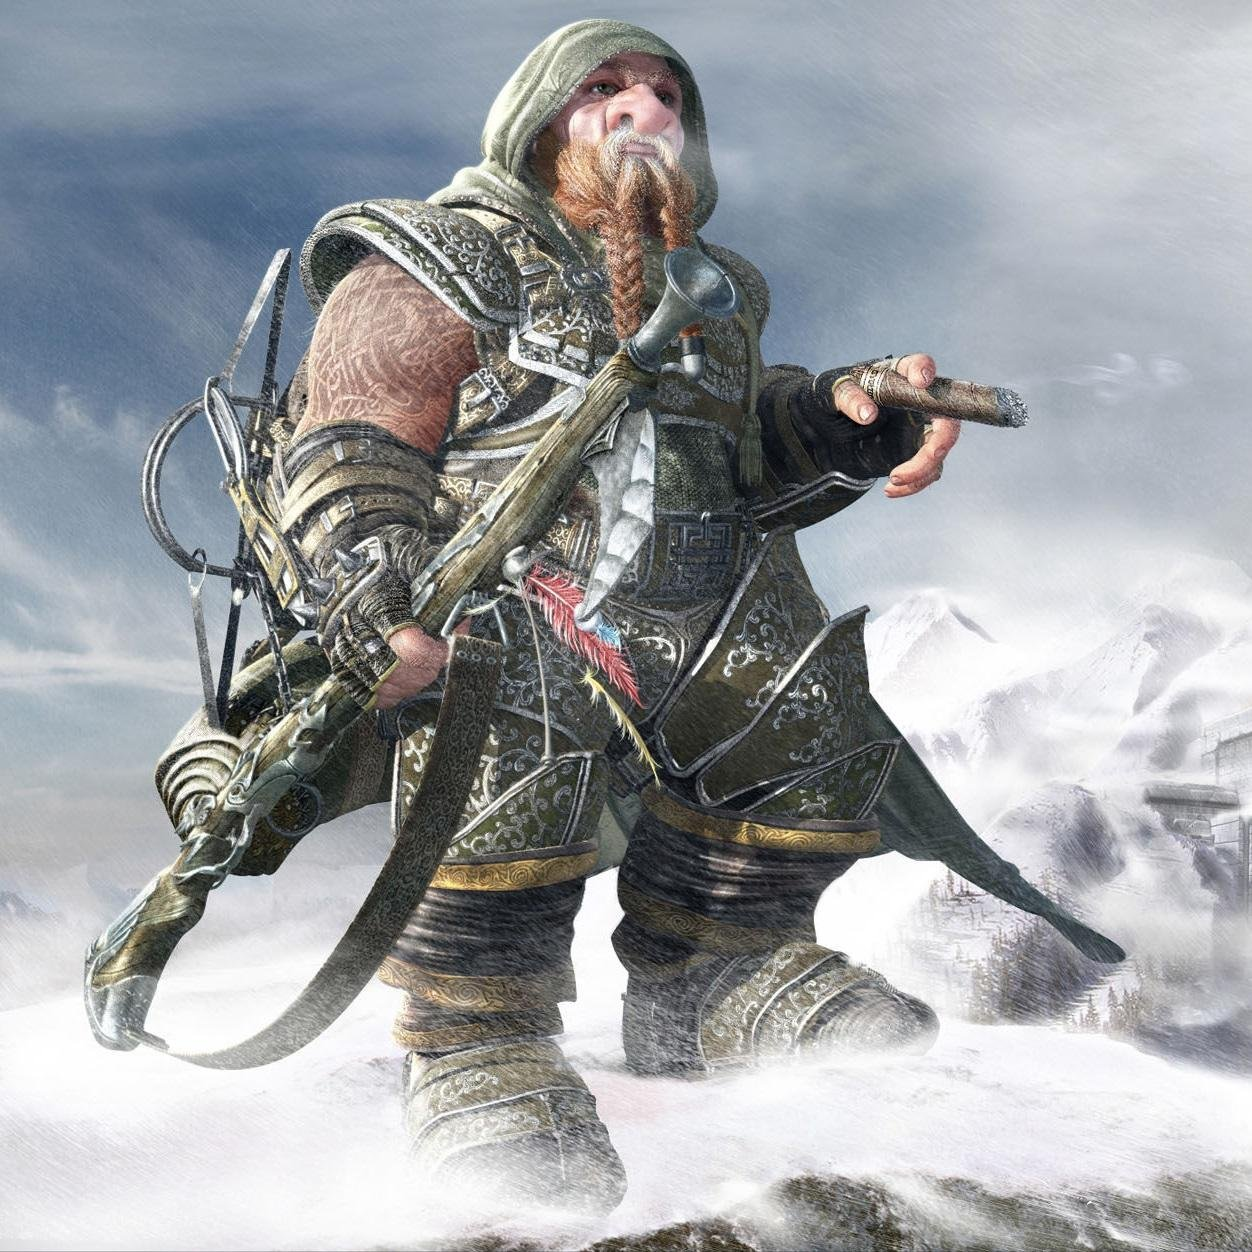
\includegraphics[width=80mm]{./content/img/riphard1.jpg}
\begin{figure}[h]
\end{figure}
\end{center}

\subsection*{Details}

\noindent

Race: 	Dwarf \\
Class: 	Pastor \\
Age: 	58 \\
Status: Active

\subsubsection{Background}

A dwarven pastor from the south, Riphard was killed by a member of the Inquisition before being resurrected by Lazarus and recruited into the mission to break the seal of the Seven.  His family, the Hardstones (or Hardthrusts), are an old dwarven dynasty from the Tom'ardy Mountains, though Riphard had long since left home to pursue his pastoral calling.

Before his death, Riphard was a man of the Church --- a true believer who preached the word of the Seven.  His encounter with Hell and subsequent resurrection shattered his faith and set him on a path of righteous vengeance against the very institution he once served.

\subsubsection{Personality and Traits}

Riphard is a hard-drinking, gun-toting dwarf with a talent for entrepreneurship and a flair for the dramatic.  Known for his thunderous whip attacks, his beloved firearms, and his tendency to launch into inspired sermons at the most inappropriate moments, Riphard is simultaneously the group's moral compass and its loosest cannon.

Despite his gruff exterior, Riphard has shown genuine tenderness --- his laying of hands on the fallen Otoria lasted ``a little too long'', and his tears upon learning he could train with the masters at the Sanctuary of Novetta were ``genuinely touching''.  He is fiercely protective of his companions, even if he would never admit it.

Riphard is also a shrewd businessman.  He founded the first bank in Velterra --- Northern Rock --- out of an old man's house in Riverfall, and later established the Guild of Banking in Hope's Rest.  His sales pitch for ``Safe Storage for a Dangerous World'' convinced even the sceptical Guild of Coin to invest.

\subsubsection{Relationships}

Riphard married Delilah Hardstone (n\'{e}e of the Jennies) and the two had twin children together, blessed by the gods and believed to possess special powers.

His relationship with the goblins has always been complicated.  An admitted anti-goblin racist early on, Riphard gradually developed a grudging respect for the twins, particularly Exme's engineering genius and Kolo's tactical cunning --- though he and Kolo clashed frequently over business ethics, lemon theft, and the proper treatment of prisoners.

Riphard earned the respect of Arbiter Kiros, who recognised his potential and recommended him for advanced training.  He also formed an unlikely bond with Pilcheur, the two sharing quiet moments of mutual understanding between bouts of mutual suspicion.

\subsubsection{Riphard's Story}

Riphard's journey took him from resurrection in Lazarus's office to becoming one of the most influential figures in Velterra.  He helped clear the Temple of Unthala, survived the Die Hard heist at the Tower of Imota Kan, founded a banking empire, crossed the Great Expanse, and fought alongside his companions through the jungles of South Africa and the civil war of Masuda.

In Masuda, Riphard acquired the legendary Hammer of the Gods from the Golden Hall --- a weapon said to have felled an Inthun-infused Varg in a single blow.  His return to the Tom'ardy Mountains revealed the ugly truth of dwarven society: a classist, slave-dependent economy built on the backs of ``Delvers'' --- miners sent on one-way trips into the deep.  His own uncle, Targon Hardthrust, had become one of them.

\clearpage
